\documentclass[11pt]{article}

\usepackage[margin=1in]{geometry}
\usepackage[T1]{fontenc}
\usepackage[utf8]{inputenc}
\usepackage{lmodern}
\usepackage{microtype}
\usepackage{amsmath,amssymb}
\usepackage{booktabs}
\usepackage{multirow}
\usepackage{xcolor}
\usepackage{graphicx}
\usepackage{caption}
\usepackage{subcaption}
\usepackage{algorithm}
\usepackage{algpseudocode}
\usepackage{pgfplots}
\pgfplotsset{compat=1.18}
\usepgfplotslibrary{fillbetween}
\usepackage[numbers,sort&compress]{natbib}
\usepackage[colorlinks=true,linkcolor=blue!50!black,citecolor=blue!50!black,urlcolor=blue!50!black]{hyperref}

\newcommand{\best}[1]{\textbf{#1}}
\newcommand{\loo}{\textsc{loo}}

\title{Citation Heads: Self-Calibrated Source Attribution\\for Cache-Augmented Generation}
\author{Ahmed Ousama\\\texttt{contact.ahmedousama@gmail.com}}
\date{}

\begin{document}
\maketitle

\begin{abstract}
Cache-augmented generation (CAG) answers questions from a knowledge base that a language model has read once into its key--value (KV) cache, but its answers come without sources and without a sign of when they are wrong. We show that both can be read from the model cheaply, by letting an expensive signal teach a cheap one. Hiding a document from the cache through the attention mask gives a leave-one-out signal without re-encoding anything; from about 20 questions the model writes itself, we keep the eight attention heads that agree with it best. These citation heads rank documents in one pass, need no labels and calibrate in minutes. Across 11 open models from five families, the top citation is a supporting paragraph for 74--96\% of HotpotQA answers. The heads beat the signal that selected them, match AT2's top citation while finding both supporting paragraphs more often at a quarter of its cost, transfer to MuSiQue and to Arabic, and switching them off leaves the model nearly blind to its knowledge. Most wrong answers, however, come from the knowledge itself, and asking whether the knowledge states an answer barely detects them. Taught instead by whether the model's own thinking answer agrees, again without reference answers, a linear read-out of its internal state detects wrong answers in one pass with AUROC 0.80 on held-out HotpotQA questions and 0.74--0.77 on MuSiQue and SQuAD, and lets the model think only where it helps, recovering most of the gain of always thinking at a third of the cost. A smaller model that cannot teach itself learns from a larger one. Both are released in \emph{mantiq}, an open-source CAG library.\footnote{\url{https://github.com/Ahmed-Ousama/mantiq}}
\end{abstract}

\section{Introduction}
\label{sec:intro}

Retrieval-augmented generation (RAG) retrieves a few chunks of a knowledge base for every question~\citep{lewis2020rag}. When the knowledge base fits in the model's context window, cache-augmented generation (CAG) skips retrieval altogether: the model reads the whole knowledge base once, its KV cache is kept, and each question only processes its own tokens on top of that cache~\citep{chan2024dontdorag}. Every answer sees all of the knowledge, and answering is fast; in our library, the first token of an answer about a 2{,}355-token product catalog arrives 65 times sooner than when the catalog is read again for every question.

What CAG gives up is provenance. A RAG system can at least show the chunks it retrieved; a CAG answer is conditioned on everything at once, so it does not say which document it comes from, nor whether it comes from the knowledge at all. Context attribution methods recover this, but at a cost. Leave-one-out ablation and its sparse variants run the model again with parts of the context removed, once per document or per random ablation~\citep{cohenwang2024contextcite,liu2025attribot}. AT2~\citep{cohenwang2025at2} replaces these runs with a learned combination of attention heads, but the weights are trained per model on ablation data from thousands of examples, so it only covers models for which someone has trained an estimator.

We observe that a KV cache already holds what attribution needs. First, documents can be hidden from a cached prefix through the attention mask, so a leave-one-out score needs one forward pass over the question and answer per document, with nothing re-encoded. Second, this cheap but noisy signal is enough to find, without any labels, a handful of attention heads that point at the source of an answer. We call them \emph{citation heads}. The model writes about 20 questions about its own knowledge, answers each one from the cache, and we keep the heads whose most-attended document most often agrees with the leave-one-out winner. At inference, these heads rank the documents in a single pass, however many documents there are.

Our contributions are:
\begin{itemize}
\item \textbf{Cache-native leave-one-out} attribution for CAG, which hides documents from a cached knowledge base through the attention mask (\S\ref{sec:loo}).
\item \textbf{Self-calibrated citation heads}, selected by their agreement with that signal on questions the model writes itself (\S\ref{sec:heads}). Calibration takes minutes on one consumer GPU and needs no labels, and we ship heads for 11 models from five families.
\item \textbf{An evaluation} on HotpotQA, SQuAD, MuSiQue and Arabic ARCD questions (\S\ref{sec:results}). Citation heads beat their own teacher, need about five calibration questions, match AT2's top citation at a quarter of its cost while finding both supporting paragraphs more often, and transfer across languages. Switching off the top 32 of them leaves the model nearly blind to its knowledge (accuracy 67.5\% $\to$ 26.0\%, against about 60\% for random heads from the same layers and 52.0\% for the top 32 retrieval heads), and they find both supporting paragraphs more often than retrieval heads. Analyzing them shows that in Gemma~3 every selected head lies in a global-attention layer, and that within the Qwen3 family, models of the same depth select largely the same heads.
\item \textbf{An answer check taught by thinking} (\S\ref{sec:supported}). A verification question flags answers that do not come from the knowledge but not wrong answers that the knowledge states; a linear read-out of the model's internal state, trained without labels on agreement with the model's own thinking answers, does, transfers to other datasets, and decides when to spend thinking.
\item \textbf{Practical lessons} for KV-cache reuse: two failure modes we hit while calibrating, chunked prefill with length-dependent rotary embeddings and thinking-mode chat templates, and an exact incremental cache update (\S\ref{sec:failures}, \S\ref{sec:updates}). All of it is released as the open-source library \emph{mantiq}.
\end{itemize}

\section{Related Work}
\label{sec:related}

\paragraph{Cache-augmented generation and KV reuse.} \citet{chan2024dontdorag} propose CAG as an alternative to RAG for knowledge bases that fit in context. Reusing the KV cache of a shared prefix is also standard in serving systems, through automatic prefix caching in vLLM~\citep{kwon2023vllm} and RadixAttention in SGLang~\citep{zheng2024sglang}; Prompt Cache~\citep{gim2024promptcache} and CacheBlend~\citep{yao2025cacheblend} reuse the KV states of separately encoded modules or chunks. Our incremental update is a form of prefix reuse; our focus is on what a cached knowledge base enables beyond speed.

\paragraph{Context attribution.} Attribution can be generated, by prompting or training models to cite~\citep{gao2023alce,zhang2024longcite}, or measured on a fixed answer. ContextCite~\citep{cohenwang2024contextcite} fits a sparse linear surrogate to the answer's likelihood under random context ablations, and AttriBoT~\citep{liu2025attribot} approximates leave-one-out attribution efficiently with cached activations, hierarchical attribution and smaller proxy models; our cache-native leave-one-out goes further and re-encodes nothing after the hidden document, which is cheaper but approximate. AT2~\citep{cohenwang2025at2} treats the attention weights of every head as features and learns per-model coefficients that predict ablation effects, from 2{,}000 training examples with 32 ablations each. It is the closest work to ours, and we compare with its released estimators in \S\ref{sec:at2}. MIRAGE~\citep{qi2024mirage} attributes answers with saliency over model internals, and \citet{basu2025circuits} attribute extractive answers with a single head found through circuit analysis. Evaluation frameworks for attribution include AIS~\citep{rashkin2023ais} and attributed QA~\citep{bohnet2022aqa}.

\paragraph{Attention heads with a function.} Only a few heads matter for many behaviors~\citep{voita2019heads,michel2019sixteen}, and some implement identifiable mechanisms such as induction~\citep{olsson2022induction} or copying from a long context (retrieval heads; \citealp{wu2024retrievalhead}). Query-focused retrieval heads~\citep{zhang2025qrhead} rank passages by the attention of heads selected on a handful of labeled examples from a real task, and in-context re-ranking~\citep{chen2025icr} aggregates the attention of all heads, calibrated with a content-free query. Retrieval heads are found without labels too, from synthetic needle-in-a-haystack copying; ours come from natural questions the model writes and a causal signal, and \S\ref{sec:retrieval} compares the two directly. Attention alone is known to be an unreliable explanation~\citep{jain2019attention,wiegreffe2019attention}; using leave-one-out as the selection criterion ties the selected heads to the effect of removing a document.

\paragraph{Detecting unsupported answers.} Models can estimate whether their answers are true (P(True); \citealp{kadavath2022know}), and disagreement between sampled answers signals hallucination~\citep{manakul2023selfcheckgpt,kuhn2023semantic}. Lookback Lens~\citep{chuang2024lookback} trains a classifier on how much each head attends to the context. We compare several of these signals for answers given from a cached knowledge base.

\section{Method}
\label{sec:method}

\subsection{Setup}
The knowledge base is a list of documents $d_1,\dots,d_n$, each a name and a text. mantiq renders the model's chat template with a system instruction, the documents separated by blank lines, and a placeholder where the question goes. It runs the model once over everything before the placeholder, in chunks of 1{,}024 tokens, and keeps the KV cache $C$ along with the token span $S_i$ of each document. To answer a question $q$, it feeds the tokens of $q$ and the rest of the chat turn on top of $C$, generates an answer $a = (a_1,\dots,a_m)$ greedily, and crops the cache back to $C$. We write $\ell(a) = \frac{1}{m}\log p(a \mid C, q)$ for the answer's mean log-probability per token.

\subsection{Leave-one-out on a cached knowledge base}
\label{sec:loo}
To measure how much the answer depends on document $i$, we hide it: in a forward pass over $q$ and $a$ on top of $C$, the attention mask is set to zero for the keys in $S_i$. Positions are left unchanged and nothing is re-encoded. The leave-one-out score is
\begin{equation}
\Delta_i = \ell(a) - \ell_{\setminus S_i}(a),
\end{equation}
the drop in log-probability per token when $d_i$ is hidden. Ranking $n$ documents costs $n+1$ passes over the $|q|+m$ question and answer tokens, compared with $n+1$ passes over the whole context when documents are removed and the context is read again. The hiding is approximate: documents after $d_i$ were encoded while $d_i$ was visible, so their cached states may still carry some of its content. With many documents, mantiq only hides the 16 documents that receive the most attention.

\subsection{Self-calibrated citation heads}
\label{sec:heads}
\paragraph{Attention per document.} For each layer $l$ and query head $h$, let $\alpha^{(l,h)}_{t,j}$ be the attention from position $t$ to key $j$. We sum it over the positions $T$ whose outputs predict the answer tokens, from the last token before the answer to $a_{m-1}$, and over each document's span, then normalize over documents:
\begin{equation}
A^{(l,h)}_i = \sum_{t \in T} \sum_{j \in S_i} \alpha^{(l,h)}_{t,j}, \qquad s^{(l,h)}_i = \frac{A^{(l,h)}_i}{\sum_k A^{(l,h)}_k}.
\end{equation}
We compute this inside a custom attention function registered with the transformers library~\citep{wolf2020transformers}, in float32, for the question and answer rows only, so the full attention matrix is never stored.

\paragraph{Calibration.} Algorithm~\ref{alg:calibrate} picks the heads. The model writes one short question about each of $Q$ documents spread over a calibration cache, without seeing the cache; it answers each question from the cache; and for each answer we compute $\Delta$ and $s$. A head scores one point when its most-attended document is the document whose hiding hurts the answer most, and its mean share on that document breaks ties. We keep the $k$ best heads, by default $k=8$ and $Q=20$ on a cache of 40 documents. No reference answers or document labels are used: the model's own leave-one-out signal is the only supervision.

\begin{algorithm}[t]
\caption{Calibrating citation heads}
\label{alg:calibrate}
\begin{algorithmic}[1]
\Require cache $C$ of documents $d_1,\dots,d_n$; number of questions $Q$; number of heads $k$
\State $g^{(l,h)} \gets 0$, $\bar{s}^{(l,h)} \gets 0$ for every head
\For{$Q$ documents $d$ spread over $C$}
  \State $q \gets$ question the model writes about $d$ (without $C$)
  \State $a \gets$ the model's answer to $q$ from $C$
  \State $s \gets$ per-head attention shares of $a$ over the documents \Comment{one pass}
  \State $i^\star \gets \arg\max_i \Delta_i$ \Comment{$n$ passes with one document hidden}
  \State $g^{(l,h)} \gets g^{(l,h)} + \mathbb{1}[\arg\max_i s^{(l,h)}_i = i^\star]$; \quad $\bar{s}^{(l,h)} \gets \bar{s}^{(l,h)} + s^{(l,h)}_{i^\star}$
\EndFor
\State \Return the $k$ heads with the highest $g^{(l,h)} + \bar{s}^{(l,h)} / (Q+1)$
\end{algorithmic}
\end{algorithm}

\paragraph{Citing.} Given the heads $H$, documents are ranked by $\sum_{(l,h)\in H} s^{(l,h)}_i$, from a single pass over $q$ and $a$. For the top $k$ documents mantiq also reports $\Delta_i$ as a score, which costs $k$ more passes; all timings below include these passes and the verification score of \S\ref{sec:supported-method}.

\subsection{A verification score}
\label{sec:supported-method}
To flag answers that do not come from the knowledge, mantiq asks the model a follow-up question over the same cache: the question, the proposed answer, and ``Is the proposed answer stated in the context? Reply with yes or no.'' The score \texttt{supported} is $P(\text{yes})/(P(\text{yes})+P(\text{no}))$ at the first answer token, summed over the casing and leading-space variants of each word that the tokenizer produces.

\subsection{Incremental updates}
\label{sec:updates}
When documents change, mantiq renders the new prompt, finds the longest common prefix of the new and cached token sequences, crops the cache to it, and reads only the remaining tokens. Because attention is causal, the result is the same cache that a fresh read would produce; our tests check this tensor by tensor, including after an interrupted update. Putting the documents that change often last makes updates cheap: changing the last document of a 964-token catalog takes 0.3\,s instead of 11.8\,s for a rebuild with Qwen3-0.6B on a laptop CPU.

\section{Experimental Setup}
\label{sec:setup}

\paragraph{Models.} We evaluate 11 instruction-tuned models: Qwen3 0.6B, 1.7B, 4B and 8B~\citep{qwen3}, Llama~3.2 1B and 3B and Llama~3.1 8B~\citep{llama3}, Gemma~3 1B and 4B~\citep{gemma3}, Mistral-7B-Instruct-v0.3~\citep{mistral7b} and Phi-4-mini-instruct~\citep{phi4mini}. The 7B and 8B models run in 4-bit NF4~\citep{dettmers2023qlora}; the others in float16 or float32 (Gemma-3-4B produced non-finite values in float16). Qwen3 answers with thinking disabled. All runs use a single NVIDIA T4 GPU (16\,GB) on Kaggle, except Gemma-3-4B in float32, which is split over two.

\paragraph{Data.} \emph{HotpotQA}~\citep{yang2018hotpotqa}: questions from the distractor validation set, excluding yes/no questions, with their 10 paragraphs, of which 2 are labeled as supporting; a harder variant pads the context to 100 paragraphs with paragraphs from other questions (about 13{,}000 tokens). \emph{SQuAD}~\citep{rajpurkar2016squad}: validation questions with their paragraph and 9 others. \emph{MuSiQue-Ans}~\citep{trivedi2022musique}: 20 paragraphs per question, 2 to 4 of them supporting. \emph{ARCD}~\citep{mozannar2019arcd}: Arabic questions with their paragraph and 9 others, with the instructions in Arabic. Each question gets its own cache, with paragraphs in random order. The calibration cache holds 40 HotpotQA paragraphs that no test question uses.

\paragraph{Protocol.} The system instruction is ``You answer questions using only the given context.'' and the answer instruction ``Answer with a short phrase only.'' Answers are greedy, with at most 24 new tokens. An answer is correct when a normalized reference answer is a substring of it. Citations are evaluated for every answer, correct or not, against the dataset's labels.

\paragraph{Metrics.} \emph{Top-1}: the top-ranked document is a supporting one. \emph{Both@2} (HotpotQA): both supporting paragraphs are among the top two. \emph{Recall@$|G|$} (MuSiQue): the fraction of the $|G|$ supporting paragraphs found among the top $|G|$. Random ranking gives a top-1 of 20\% and a both@2 of 2.2\% on HotpotQA. We report 95\% bootstrap confidence intervals (4{,}000 resamples), paired for differences between methods on the same answers. With 80 questions per model, intervals on top-1 are about $\pm$7 points, so we rely on the paired intervals and on consistency across models.

\paragraph{Baselines.} \emph{Leave-one-out} (\loo): \S\ref{sec:loo}, hiding every document (with 100 documents, the 16 most attended). \emph{AT2}~\citep{cohenwang2025at2}: the authors' released estimators for Llama-3.1-8B-Instruct and Phi-4-mini-instruct, applied with their code to the exact text the model saw and the same answers. The Llama estimator was trained on the full-precision model and runs here on the 4-bit one.

\section{Results}
\label{sec:results}

\subsection{Citation heads across models}

\begin{table}[t]
\centering
\small
\caption{Citation accuracy (\%) without (\loo) and with citation heads, on the same answers. HotpotQA: 80 questions per model (150 for Qwen3-4B and Phi-4-mini); SQuAD: 40 (150 for Qwen3-4B). Time: seconds per cited answer with 10 paragraphs, including the verification score. Calib.: seconds to calibrate. 4b: 4-bit NF4.}
\label{tab:models}
\setlength{\tabcolsep}{4.5pt}
\begin{tabular}{llrrrrrrrrr}
\toprule
& & & \multicolumn{2}{c}{HotpotQA top-1} & \multicolumn{2}{c}{HotpotQA both@2} & \multicolumn{2}{c}{SQuAD top-1} & \multicolumn{2}{c}{Time (s)} \\
\cmidrule(lr){4-5}\cmidrule(lr){6-7}\cmidrule(lr){8-9}\cmidrule(lr){10-11}
Model & Prec. & Calib. & \loo & heads & \loo & heads & \loo & heads & \loo & heads \\
\midrule
Qwen3-0.6B & fp32 & 124 & 68.8 & \best{73.8} & \best{33.8} & 30.0 & 95.0 & \best{97.5} & 0.63 & \best{0.22} \\
Qwen3-1.7B & fp32 & 160 & 81.2 & \best{87.5} & 30.0 & \best{40.0} & 97.5 & \best{100} & 1.16 & \best{0.38} \\
Qwen3-4B & fp16 & 181 & 87.3 & \best{92.7} & 42.7 & \best{56.0} & 98.0 & \best{99.3} & 0.96 & \best{0.33} \\
Qwen3-8B & 4b & 219 & 88.8 & \best{92.5} & 37.5 & \best{45.0} & 100 & 100 & 1.75 & \best{0.59} \\
Llama-3.2-1B & fp32 & 85 & 88.8 & 88.8 & 28.7 & \best{41.2} & 90.0 & \best{97.5} & 0.70 & \best{0.24} \\
Llama-3.2-3B & fp16 & 99 & \best{95.0} & 93.8 & 48.8 & \best{53.8} & 97.5 & \best{100} & 0.66 & \best{0.23} \\
Llama-3.1-8B & 4b & 178 & 93.8 & \best{96.2} & 47.5 & \best{53.8} & 100 & 100 & 1.56 & \best{0.54} \\
Gemma-3-1B & fp32 & -- & 74.0 & \best{77.5} & 15.0 & \best{27.5} & 92.5 & \best{97.5} & -- & -- \\
Gemma-3-4B & fp32 & 232 & 86.2 & \best{92.5} & 25.0 & \best{53.8} & 100 & 100 & 1.95 & \best{0.70} \\
Mistral-7B-v0.3 & 4b & -- & 86.0 & \best{91.0} & 40.0 & \best{54.0} & 97.5 & \best{100} & -- & -- \\
Phi-4-mini & fp16 & -- & 89.3 & \best{90.0} & 34.0 & \best{52.7} & -- & -- & 0.78 & \best{0.27} \\
\bottomrule
\end{tabular}
\end{table}

Table~\ref{tab:models} compares citation heads with leave-one-out on the same answers. Citation heads give a higher top-1 on HotpotQA for 9 of the 11 models (one tie, one point lower for Llama-3.2-3B) and a higher both@2 for 10 of 11, by 3.4 and 11.3 points on average. Per-model intervals are wide, but several paired differences exclude zero: for Qwen3-4B, $+5.3$ [0.7, 10.0] on top-1 and $+13.3$ [4.0, 22.7] on both@2; for Gemma-3-4B, $+6.2$ [1.2, 11.2] and $+28.7$ [17.5, 40.0]; for Llama-3.2-1B, $+12.5$ [1.2, 23.8] on both@2. On SQuAD, where each question has one relevant paragraph, the heads put it first for 97.5--100\% of answers. Citing with heads is also about three times faster, since one attention pass and two scoring passes replace ten hidden-document passes. Calibration takes 85 to 232 seconds per model.

\paragraph{More documents.} With 100 HotpotQA paragraphs per question (40 questions, about 13{,}000 tokens), Qwen3-4B's top citation is supporting for 90.0\% [80.0, 97.5] of answers with heads, against 77.5\% [65.0, 90.0] for leave-one-out over the 16 most attended paragraphs, and a cited answer takes 1.15\,s instead of 4.97\,s. Heads keep their cost at one pass however many documents there are, while hiding has to shortlist.

\paragraph{Another language.} On 150 ARCD questions with Arabic instructions, Qwen3-4B's built-in heads, calibrated on English questions, put the right paragraph first for 98.0\% [95.3, 100] of answers, compared with 96.0\% for leave-one-out and 98.7\% for heads calibrated on Arabic questions.

\subsection{Comparison with AT2}
\label{sec:at2}

\begin{table}[t]
\centering
\small
\caption{Citation heads vs.\ AT2 and leave-one-out on the same 150 HotpotQA answers per model, with 95\% bootstrap intervals. The last row of each model is the paired difference between heads and AT2.}
\label{tab:at2}
\begin{tabular}{llccr}
\toprule
Model & Method & Top-1 (\%) & Both@2 (\%) & Time (s) \\
\midrule
\multirow{4}{*}{Llama-3.1-8B (4b)} & citation heads & \best{92.7} [88.0, 96.7] & \best{58.0} [50.0, 66.0] & \best{0.53} \\
& AT2 & 92.0 [87.3, 96.0] & 44.0 [36.0, 52.0] & 1.98 \\
& leave-one-out & 92.7 [88.0, 96.7] & 46.7 [39.3, 54.7] & 1.54 \\
& \emph{heads $-$ AT2} & $+0.7$ [$-2.0$, 4.0] & $+14.0$ [7.3, 20.7] & \\
\midrule
\multirow{4}{*}{Phi-4-mini (fp16)} & citation heads & \best{90.0} [84.7, 94.7] & \best{52.7} [44.7, 60.7] & \best{0.27} \\
& AT2 & 87.3 [82.0, 92.7] & 45.3 [37.3, 53.3] & 1.16 \\
& leave-one-out & 89.3 [84.0, 94.0] & 34.0 [26.7, 41.3] & 0.78 \\
& \emph{heads $-$ AT2} & $+2.7$ [$-1.3$, 6.7] & $+7.3$ [1.3, 14.0] & \\
\bottomrule
\end{tabular}
\end{table}

Table~\ref{tab:at2} compares citation heads with AT2's released estimators on identical inputs and answers. For the top citation the three methods are on par: the paired differences between heads and AT2 are within $[-2.0, 6.7]$ points. For both@2, citation heads are ahead of AT2 by 14.0 points on Llama-3.1-8B and 7.3 points on Phi-4-mini, with paired intervals above zero. They are also 3.7 and 4.3 times faster in our setup, where AT2 runs its own forward pass with attention weights while citation heads collect the attention during the pass that also scores the answer. AT2's estimators come from 64{,}000 ablated forward passes per model (2{,}000 examples with 32 ablations each); citation heads come from 20 questions the model wrote itself.

\subsection{MuSiQue}
\label{sec:musique}

\begin{table}[t]
\centering
\small
\caption{MuSiQue-Ans, 20 paragraphs per question with 2 to 4 supporting (2.67 on average), 150 questions per model, with 95\% bootstrap intervals. The heads are the built-in ones, found on HotpotQA and used unchanged. Leave-one-out hides all 20 paragraphs. A random ranking scores 13.4\% on both metrics. Time: seconds per cited answer, including scores for the top 4 citations and the verification score.}
\label{tab:musique}
\begin{tabular}{llccr}
\toprule
Model & Method & Top-1 (\%) & Recall@$|G|$ (\%) & Time (s) \\
\midrule
\multirow{4}{*}{Llama-3.1-8B (4b)} & citation heads & \best{75.3} [68.7, 82.0] & \best{57.9} [53.4, 62.4] & \best{0.92} \\
& AT2 & 72.7 [66.0, 80.0] & 52.4 [47.6, 57.4] & 4.75 \\
& leave-one-out & \best{75.3} [68.0, 82.0] & 54.5 [49.5, 59.6] & 3.25 \\
& \emph{heads $-$ AT2} & $+2.7$ [$-1.3$, 6.7] & $+5.5$ [1.8, 9.3] & \\
\midrule
\multirow{4}{*}{Phi-4-mini (fp16)} & citation heads & \best{65.3} [58.0, 72.7] & \best{54.8} [49.9, 59.7] & \best{0.48} \\
& AT2 & 64.0 [56.0, 72.0] & 47.9 [42.9, 52.8] & 2.98 \\
& leave-one-out & 64.0 [56.0, 71.3] & 50.6 [45.8, 55.3] & 1.68 \\
& \emph{heads $-$ AT2} & $+1.3$ [$-2.0$, 4.7] & $+6.9$ [3.1, 10.7] & \\
\midrule
\multirow{3}{*}{Qwen3-4B (fp16)} & citation heads & \best{80.0} [73.3, 86.0] & \best{57.0} [52.1, 61.8] & \best{0.61} \\
& leave-one-out & 76.0 [68.7, 82.7] & 50.4 [46.1, 54.9] & 2.13 \\
& \emph{heads $-$ leave-one-out} & $+4.0$ [$-0.7$, 8.7] & $+6.6$ [1.8, 11.4] & \\
\bottomrule
\end{tabular}
\end{table}

MuSiQue composes 2- to 4-hop questions from single-hop ones, so most answers depend on several paragraphs and shortcuts are rarer than in HotpotQA~\citep{trivedi2022musique}. It is also a test of transfer: the built-in heads were found on HotpotQA paragraphs and are used unchanged. Table~\ref{tab:musique} shows the same picture as on HotpotQA. For the top citation, citation heads are on par with or ahead of AT2 and leave-one-out on all three models. For recall of all supporting paragraphs they are ahead of AT2 by 5.5 points on Llama-3.1-8B and 6.9 points on Phi-4-mini, and of leave-one-out by 6.6 points on Qwen3-4B, with paired intervals above zero, while being 3.5 to 6.2 times faster than either. The models answer only 23--35\% of these questions correctly; the citations are evaluated for every answer, and the advantage of the heads in recall holds among the wrong answers (58\% vs.\ 49\% for both AT2 and leave-one-out on Llama-3.1-8B).

\subsection{What makes citation heads work}
\label{sec:ablations}

We saved the per-head attention shares and the leave-one-out scores of Qwen3-4B for 30 calibration questions (HotpotQA, 10 paragraphs, disjoint from the test questions) and for test sets of HotpotQA with 10 (150 questions) and 100 paragraphs (60), and SQuAD with 10 (150) and 100 paragraphs (60). This allows any head selection to be evaluated offline (Table~\ref{tab:ablation}, Figure~\ref{fig:calibration}).

\begin{table}[t]
\centering
\small
\caption{Head selection for Qwen3-4B, evaluated offline on saved attention shares (top-1 \%). Heads are selected on 30 HotpotQA questions unless stated otherwise.}
\label{tab:ablation}
\begin{tabular}{lcccc}
\toprule
& \multicolumn{2}{c}{HotpotQA} & \multicolumn{2}{c}{SQuAD} \\
\cmidrule(lr){2-3}\cmidrule(lr){4-5}
Ranking & 10 par. & 100 par. & 10 par. & 100 par. \\
\midrule
random & 22.7 & 0.0 & 11.3 & 3.3 \\
all 1{,}152 heads, mean share & 21.3 & 23.3 & 47.3 & 53.3 \\
all heads, total attention & 59.3 & 43.3 & 97.3 & 86.7 \\
leave-one-out (the calibration signal) & 86.7 & 80.0 & 98.0 & 95.0 \\
\midrule
8 heads, selected with leave-one-out labels & 92.0 & 86.7 & 99.3 & 98.3 \\
8 heads, selected with gold labels & 92.0 & 86.7 & 99.3 & 98.3 \\
8 built-in heads (20 self-written questions) & \best{92.7} & \best{88.3} & 99.3 & 98.3 \\
\midrule
1 head & 83.3 & 71.7 & 99.3 & 98.3 \\
2 heads & \best{92.7} & \best{88.3} & 99.3 & 98.3 \\
32 heads & 92.0 & 86.7 & 99.3 & 98.3 \\
128 heads & 91.3 & 85.0 & 99.3 & 98.3 \\
\bottomrule
\end{tabular}
\end{table}

\paragraph{Selection is what matters.} Averaging the attention shares of all 1{,}152 heads ranks HotpotQA paragraphs barely better than chance (21.3\%), and summing raw attention reaches 59.3\%. Any small selected set, from 2 to 128 heads, reaches 91--93\%; a single head already reaches 83\%.

\paragraph{The student beats the teacher.} The heads are selected to agree with leave-one-out, yet they are more accurate than leave-one-out itself: 92.0\% vs.\ 86.7\% with 10 paragraphs and 86.7\% vs.\ 80.0\% with 100. Leave-one-out is noisy on multi-hop questions: when the answer is stated in one paragraph but the question also needs another, hiding either may change the answer's probability little, and hiding a distractor that shares the answer's entity can change it a lot. Selection aggregates leave-one-out over many questions and keeps the heads that agree with it consistently, so per-question noise averages out, while the selected heads attend to where the answer is read from.

\paragraph{No labels needed.} Selecting heads by agreement with gold supporting paragraphs instead of leave-one-out gives the same top-1 on all four test sets. The heads built into mantiq, selected from 20 questions that the model wrote without seeing any labels, are as good or better.

\paragraph{Five questions are enough.} Figure~\ref{fig:calibration} varies the number of calibration questions over 100 random subsets. With one or two questions the selection is unstable. With five, the mean top-1 is within 1.1 points of using all 30 questions on 10 paragraphs (3.4 on 100) and above leave-one-out on both; from eight questions on, at least 90\% of the subsets beat leave-one-out on both test sets.

\begin{figure}[t]
\centering
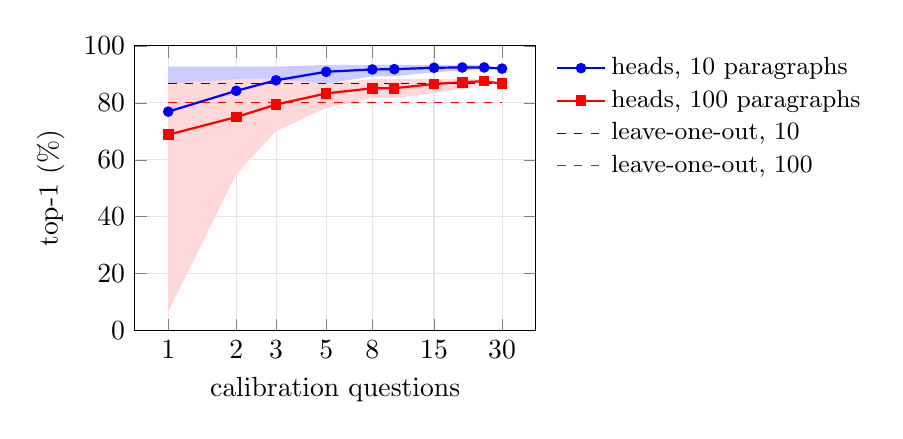
\begin{tikzpicture}
\begin{axis}[
  width=0.55\linewidth, height=5.2cm,
  xlabel={calibration questions}, ylabel={top-1 (\%)},
  xmode=log, log basis x=2, xtick={1,2,3,5,8,15,30}, xticklabels={1,2,3,5,8,15,30},
  ymin=0, ymax=100, legend pos=outer north east, legend style={font=\small, draw=none}, legend cell align=left,
  grid=major, grid style={gray!20},
]
\addplot[name path=h10hi, draw=none, forget plot] coordinates {(1,92.7)(2,92.7)(3,92.7)(5,93.3)(8,93.3)(10,93.3)(15,93.3)(20,93.3)(25,93.3)(30,92.0)};
\addplot[name path=h10lo, draw=none, forget plot] coordinates {(1,23.3)(2,72.7)(3,80.7)(5,86.7)(8,89.3)(10,89.3)(15,90.7)(20,91.3)(25,92.0)(30,92.0)};
\addplot[blue!20, forget plot] fill between[of=h10hi and h10lo];
\addplot[blue, thick, mark=*, mark size=1.5pt] coordinates {(1,76.9)(2,84.2)(3,87.9)(5,90.9)(8,91.7)(10,91.8)(15,92.3)(20,92.4)(25,92.4)(30,92.0)};
\addlegendentry{heads, 10 paragraphs}
\addplot[name path=h100hi, draw=none, forget plot] coordinates {(1,86.7)(2,88.3)(3,88.3)(5,86.7)(8,88.3)(10,88.3)(15,88.3)(20,88.3)(25,88.3)(30,86.7)};
\addplot[name path=h100lo, draw=none, forget plot] coordinates {(1,6.7)(2,55.0)(3,70.0)(5,78.3)(8,81.7)(10,81.7)(15,83.3)(20,85.0)(25,86.7)(30,86.7)};
\addplot[red!15, forget plot] fill between[of=h100hi and h100lo];
\addplot[red, thick, mark=square*, mark size=1.5pt] coordinates {(1,68.8)(2,75.0)(3,79.4)(5,83.3)(8,85.1)(10,85.1)(15,86.6)(20,87.2)(25,87.6)(30,86.7)};
\addlegendentry{heads, 100 paragraphs}
\addplot[blue, dashed, domain=1:30, samples=2] {86.7};
\addlegendentry{leave-one-out, 10}
\addplot[red, dashed, domain=1:30, samples=2] {80.0};
\addlegendentry{leave-one-out, 100}
\end{axis}
\end{tikzpicture}
\caption{Top-1 on HotpotQA for Qwen3-4B against the number of calibration questions (mean over 100 random subsets; bands from the 10th to the 90th percentile). Dashed lines: leave-one-out, the signal the heads are calibrated on.}
\label{fig:calibration}
\end{figure}

\paragraph{Where the heads are.} Figure~\ref{fig:depth} shows the built-in heads of all 11 models. They sit mostly in the middle and upper-middle layers (median at 61\% of the depth). Two patterns stand out. In both Gemma~3 models, all 16 selected heads are in global-attention layers (layers 5, 11, 17, 23 and 29, one in six; the others attend within a sliding window), although nothing in the selection knows about the architecture: heads that can only see the last window of tokens cannot reach most documents. And within the Qwen3 family, models of the same depth select largely the same heads: 5 of 8 are shared between Qwen3-0.6B and 1.7B (28 layers each), and 4 of 8 between Qwen3-4B and 8B (36 layers each), out of 448 and 1{,}152 heads respectively. This is consistent with the smaller Qwen3 models being distilled from larger ones~\citep{qwen3}, though we have not tested the cause.

\begin{figure}[t]
\centering
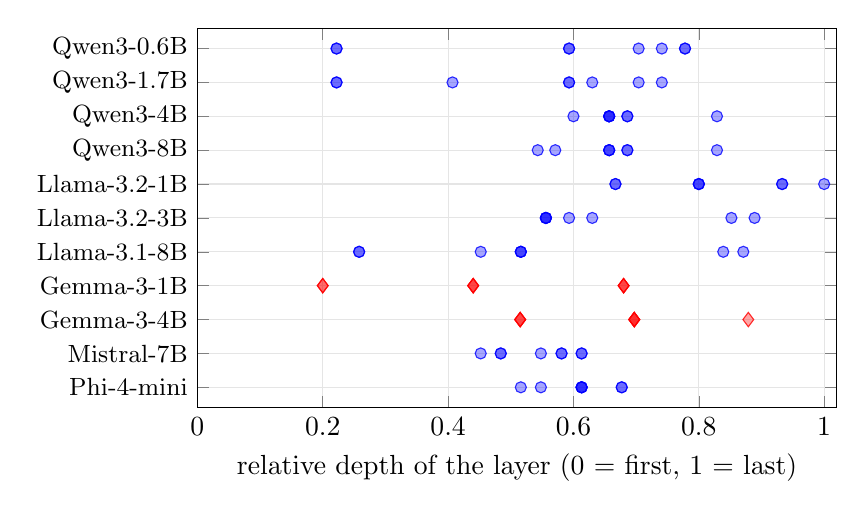
\begin{tikzpicture}
\begin{axis}[
  width=0.8\linewidth, height=6.4cm,
  xlabel={relative depth of the layer (0 = first, 1 = last)},
  xmin=0, xmax=1.02, ymin=-0.6, ymax=10.6,
  ytick={0,...,10},
  yticklabels={Phi-4-mini, Mistral-7B, Gemma-3-4B, Gemma-3-1B, Llama-3.1-8B, Llama-3.2-3B, Llama-3.2-1B, Qwen3-8B, Qwen3-4B, Qwen3-1.7B, Qwen3-0.6B},
  yticklabel style={font=\small},
  grid=major, grid style={gray!20},
]
\addplot[only marks, mark=*, mark size=2pt, fill opacity=0.35, draw opacity=0.8, blue] coordinates {
(0.613,0) (0.677,0) (0.677,0) (0.613,0) (0.548,0) (0.613,0) (0.516,0) (0.613,0)
(0.452,1) (0.548,1) (0.581,1) (0.613,1) (0.484,1) (0.581,1) (0.613,1) (0.484,1)
(0.839,4) (0.258,4) (0.516,4) (0.258,4) (0.516,4) (0.516,4) (0.452,4) (0.871,4)
(0.556,5) (0.630,5) (0.556,5) (0.852,5) (0.556,5) (0.593,5) (0.556,5) (0.889,5)
(0.800,6) (0.933,6) (0.933,6) (0.800,6) (1.000,6) (0.667,6) (0.800,6) (0.667,6)
(0.657,7) (0.657,7) (0.829,7) (0.657,7) (0.686,7) (0.686,7) (0.571,7) (0.543,7)
(0.657,8) (0.686,8) (0.657,8) (0.829,8) (0.657,8) (0.657,8) (0.686,8) (0.600,8)
(0.593,9) (0.407,9) (0.741,9) (0.222,9) (0.704,9) (0.222,9) (0.593,9) (0.630,9)
(0.593,10) (0.222,10) (0.741,10) (0.593,10) (0.778,10) (0.704,10) (0.778,10) (0.222,10)
};
\addplot[only marks, mark=diamond*, mark size=2.6pt, fill opacity=0.35, draw opacity=0.8, red] coordinates {
(0.515,2) (0.515,2) (0.515,2) (0.879,2) (0.697,2) (0.697,2) (0.697,2) (0.697,2)
(0.680,3) (0.680,3) (0.440,3) (0.200,3) (0.200,3) (0.680,3) (0.440,3) (0.440,3)
};
\end{axis}
\end{tikzpicture}
\caption{Layers of the eight built-in citation heads of each model; darker marks are layers with several selected heads. Red: Gemma~3, where every selected head is in a global-attention layer.}
\label{fig:depth}
\end{figure}

\paragraph{The heads are the model's eyes on the knowledge.} Selection by agreement with leave-one-out says that the heads look at the right document, not that the model reads through them. To test this, we switch heads off (zero their output) while Qwen3-4B reads the question and writes the answer, with the knowledge cached as usual, on 200 HotpotQA questions (Table~\ref{tab:knockout}). As controls, we switch off as many random heads from the same layers, in three draws. Switching off the top 8 citation heads costs 6.5 points of accuracy, about as much as 8 random heads (0.5 to 3 points), so other heads compensate. Switching off the top 32 makes the model nearly blind to its knowledge: accuracy falls from 67.5\% to 26.0\%, the share of answers found in the knowledge from 70\% to 17\%, and the model often replies that the context does not mention what it asks about, while 32 random heads from the same layers leave 57.5--62.5\% accuracy. This agrees with ablations of retrieval heads~\citep{wu2024retrievalhead} and in-context heads~\citep{kahardipraja2025atlas}; here the heads come from 20 questions the model wrote itself.

\begin{table}[t]
\centering
\small
\caption{Switching heads off while Qwen3-4B answers 200 HotpotQA questions from its cached knowledge. Random heads come from the same layers as the citation heads (three draws; range shown). \emph{In knowledge}: the answer appears verbatim in the paragraphs.}
\label{tab:knockout}
\begin{tabular}{lccc}
\toprule
Heads switched off & Accuracy (\%) & In knowledge (\%) & Mean \texttt{supported} \\
\midrule
none & 67.5 [60.5, 73.5] & 70 & 0.93 \\
top 8 citation heads & 61.0 [54.5, 68.0] & 68 & 0.90 \\
8 random heads & 64.5--67.0 & 58--76 & 0.91--0.92 \\
top 32 citation heads & \best{26.0} [20.5, 32.0] & \best{17} & \best{0.59} \\
32 random heads & 57.5--62.5 & 52--76 & 0.82--0.90 \\
\bottomrule
\end{tabular}
\end{table}

\paragraph{Citation heads are not retrieval heads.}
\label{sec:retrieval}
Retrieval heads~\citep{wu2024retrievalhead} are found by hiding a needle sentence in a long haystack and keeping the heads whose most-attended token is the needle token being copied. We found them the same way for Qwen3-4B and Phi-4-mini (haystacks of 1{,}000 to 4{,}000 tokens of unrelated HotpotQA paragraphs, 5 depths, 3 needles) and compared them with citation heads on the same answers (Table~\ref{tab:retrieval}). The two sets overlap only partly: 2 and 1 of the top 8 heads are shared, 9 and 15 of the top 32, and the 8 citation heads of Qwen3-4B rank between 0th and 67th of 1{,}152 heads by retrieval score. For the top citation they are on par, but citation heads find both supporting paragraphs 20.0 [13.3, 26.7] points more often on Qwen3-4B and 8.7 [1.3, 15.3] on Phi-4-mini. And switching off the top 32 citation heads hurts answers much more than switching off the top 32 retrieval heads ($-26.0$ [$-33.0$, $-19.0$] and $-15.0$ [$-21.0$, $-9.5$] points of accuracy): copying a needle and reading the documents an answer comes from rely on overlapping but different heads.

\begin{table}[t]
\centering
\small
\caption{Citation heads vs.\ retrieval heads~\citep{wu2024retrievalhead} found for the same model. Citation: 150 HotpotQA questions (10 paragraphs). Knockout: accuracy on 200 HotpotQA questions with the top 32 heads of each kind switched off while answering (no heads switched off: 67.5\% for Qwen3-4B, 57.5\% for Phi-4-mini).}
\label{tab:retrieval}
\begin{tabular}{llccc}
\toprule
Model & Heads & Top-1 (\%) & Both@2 (\%) & Accuracy, top 32 off (\%) \\
\midrule
\multirow{3}{*}{Qwen3-4B} & citation heads & 90.7 [86.0, 95.3] & \best{56.7} [48.7, 64.0] & \best{26.0} [20.0, 32.5] \\
& retrieval heads & 91.3 [86.7, 95.3] & 36.7 [28.7, 44.7] & 52.0 [45.5, 59.0] \\
& leave-one-out & 86.0 [80.7, 91.3] & 37.3 [30.0, 45.3] & \\
\midrule
\multirow{3}{*}{Phi-4-mini} & citation heads & 90.0 [84.7, 94.7] & \best{52.7} [44.7, 60.7] & \best{15.0} [10.5, 20.0] \\
& retrieval heads & 88.0 [82.7, 93.3] & 44.0 [36.0, 52.0] & 30.0 [23.5, 36.5] \\
& leave-one-out & 89.3 [84.0, 94.0] & 34.0 [26.7, 42.0] & \\
\bottomrule
\end{tabular}
\end{table}

\subsection{Failure modes found while calibrating}
\label{sec:failures}

Self-calibration is only as good as the model's behavior on the calibration cache, and two problems that silently broke it are worth reporting, since they affect any system that reuses KV caches.

\paragraph{Length-dependent rotary embeddings and chunked prefill.} Phi-4-mini uses LongRoPE~\citep{ding2024longrope,phi3}, whose rotary frequencies~\citep{su2021roformer} switch from a short to a long set of scaling factors once a forward pass reaches positions beyond the original 4{,}096-token window; dynamic NTK scaling behaves similarly. Reading a 6{,}000-token calibration cache in chunks of 1{,}024 tokens encoded the first chunks with the short factors and the rest with the long ones. On this inconsistent cache, all 20 calibration answers degenerated into repetitions (``and and and, and\dots''), heads selected from them reached only 38\% top-1, and the same happened to any long knowledge base. mantiq now reads knowledge that crosses the threshold in a single pass, and re-reads it entirely when an update crosses it; heads recalibrated this way reach 90.0\%. The same issue arises for any prefix reuse whose total length crosses the threshold.

\paragraph{Thinking templates.} With Qwen3's thinking mode on, all 20 questions the model wrote for calibration were the literal string ``\texttt{<think>}'': the question writer stops at the first line, and in thinking mode that line opens the reasoning block. mantiq now writes calibration questions with thinking disabled and strips reasoning blocks.

\section{Verifying answers against the knowledge}
\label{sec:supported}

To evaluate \texttt{supported} (\S\ref{sec:supported-method}), each HotpotQA question is answered twice: once over its own paragraphs and once over the paragraphs of another question, where the answer cannot be found. We report two AUROCs: how often an answer from the right paragraphs scores higher than one from the wrong paragraphs (\emph{made up}), and, among answers from the right paragraphs, how often a correct one scores higher than a wrong one (\emph{wrong}).

\begin{table}[t]
\centering
\small
\caption{AUROC (\%) of \texttt{supported}, with 95\% bootstrap intervals. \emph{Made up}: answers over the question's own paragraphs vs.\ another question's. \emph{Wrong}: correct vs.\ wrong answers over the question's own paragraphs. 100 questions for Qwen3, 80 for the others, 150 in Arabic. Intervals for Gemma-3-1B and Mistral are missing because their per-question outputs were lost.}
\label{tab:supported}
\begin{tabular}{lcc}
\toprule
Model & Made up & Wrong \\
\midrule
Qwen3-0.6B & 87.8 [82.9, 92.1] & 61.9 [49.9, 73.0] \\
Qwen3-1.7B & 95.3 [92.2, 97.8] & 57.2 [47.1, 67.4] \\
Qwen3-4B & 97.5 [95.3, 99.3] & 55.9 [44.9, 67.6] \\
Qwen3-8B (4b) & 90.4 [85.9, 94.2] & 69.5 [58.4, 80.4] \\
Llama-3.2-1B & 80.7 [74.0, 86.9] & 60.5 [48.7, 72.9] \\
Llama-3.2-3B & 91.0 [86.2, 95.3] & 59.9 [47.7, 72.1] \\
Llama-3.1-8B (4b) & 86.8 [80.7, 92.0] & 69.3 [56.9, 80.6] \\
Gemma-3-1B & 90 & 50 \\
Gemma-3-4B & 83.7 [77.4, 89.6] & 59.0 [46.2, 71.0] \\
Mistral-7B-v0.3 (4b) & 96 & 67 \\
Qwen3-4B, Arabic (ARCD) & 91.7 [88.0, 95.0] & 70.1 [61.6, 78.1] \\
\bottomrule
\end{tabular}
\end{table}

Table~\ref{tab:supported} shows a clear split. \texttt{supported} separates answers given without the relevant knowledge well, with AUROCs of 81--97\% in English and 92\% in Arabic. It does much worse on wrong answers given with the right knowledge (50--70\%, with intervals that often include chance): when the model picks the wrong entity from a paragraph that is in the context, the context does state that entity, and the check agrees.

\begin{table}[t]
\centering
\small
\caption{Other signals for Qwen3-4B on 150 HotpotQA questions (AUROC \%, 95\% intervals). Sampling-based signals use 6 samples.}
\label{tab:signals}
\begin{tabular}{lcc}
\toprule
Signal & Made up & Wrong \\
\midrule
\texttt{supported} (asked after the answer) & \best{97.1} [95.0, 98.9] & 56.1 [47.4, 64.7] \\
quote: the model copies the supporting sentence; fraction found & 90.3 [86.2, 94.0] & -- \\
log-probability drop with all documents hidden & 58.4 [51.7, 65.1] & -- \\
log-probability gain over a cache without documents & 49.1 [42.6, 56.0] & -- \\
mean token probability of the answer & 81.3 [76.1, 86.1] & 60.0 [50.8, 69.0] \\
minimum token probability & 87.2 [83.0, 91.1] & \best{61.9} [52.7, 70.7] \\
agreement of sampled answers~\citep{manakul2023selfcheckgpt} & 86.9 [83.0, 90.8] & 56.0 [49.9, 62.1] \\
negative entropy of sampled answers~\citep{kuhn2023semantic} & 87.8 [84.0, 91.4] & 56.0 [50.0, 62.1] \\
P(True), shown the samples~\citep{kadavath2022know} & 62.5 [56.7, 68.4] & 58.1 [49.7, 66.5] \\
\bottomrule
\end{tabular}
\end{table}

Table~\ref{tab:signals} compares other signals on Qwen3-4B. Asking whether the context states the answer is the best detector of made-up answers, ahead of copying a supporting quote, token probabilities and sampling consistency; signals based on how much the answer's likelihood depends on the documents are near chance, because a fluent made-up answer is likely with or without them. For wrong answers from the right context, none of the signals exceeds 62\%.

\subsection{Catching wrong answers that the knowledge states}
\label{sec:wrong}

\paragraph{What the wrong answers are.} Part of the difficulty is the labels. Reading the 53 answers of Table~\ref{tab:signals} that substring matching marks as wrong, we found 22 to be right (``Woody Allen'' for ``Heywood `Woody' Allen'', ``Ghana'' for ``a Ghanaian boxer'') and 9 cut short by the token limit. From here on, answers are judged by the same model with thinking on, given the question, the reference answer(s) and the supporting paragraphs; on the 139 answers we labeled by hand it agrees with us on 93\%. The 22 truly wrong answers come from the knowledge: the model stops at a step on the way (the team, not its owner; the province, not its capital), picks an entity that meets only some conditions of the question, or loses a comparison. A question about whether the knowledge states the answer cannot catch these, and asking whether the answer gives exactly what the question asks for, or whether a sentence restating the answer is true, did no better (AUROC 0.55--0.59 on 200 questions).

\paragraph{Thinking as a teacher.} What does separate them is the model's own thinking. Qwen3 can answer with or without a thinking phase; when the fast answer and the thinking answer agree, the fast one is usually right: on 600 held-out HotpotQA questions, agreement detects wrong answers with AUROC 0.78, and the model's own probability that the two answers are the same with 0.83. But this costs a thinking phase (about 300 tokens) per question, which is the expense one wants to avoid. As with citation heads, we use the expensive signal to teach a cheap one. On 2{,}000 HotpotQA training questions, we record the model's internal state in the pass over its fast answer, and fit a logistic regression that predicts the probability that its thinking answer would agree, with no reference answers involved.

\begin{table}[t]
\centering
\small
\caption{Detecting wrong answers given with the right paragraphs (AUROC \%, 95\% intervals), Qwen3-4B. Probes are trained on 2{,}000 HotpotQA training questions with the thinking teacher only, on the 4-bit model, and tested against the judge on held-out questions: 600 from HotpotQA, and 300 each from MuSiQue and SQuAD, which the probes never saw. Accuracy of the fast answers: 67.3\%, 31.7\% and 90.0\%.}
\label{tab:wrong}
\setlength{\tabcolsep}{4pt}
\begin{tabular}{lccc}
\toprule
Signal & HotpotQA & MuSiQue & SQuAD \\
\midrule
min token probability of the answer & 63.3 [58.7, 68.4] & 55.0 [47.2, 62.3] & 68.8 [58.8, 78.2] \\
P(yes) to ``is the proposed answer correct?'' & 68.5 [63.9, 72.9] & 60.0 [53.1, 66.5] & 73.7 [63.9, 83.2] \\
\texttt{supported} & 68.9 [64.0, 73.3] & 62.6 [55.7, 69.2] & 76.0 [65.1, 86.1] \\
\midrule
\emph{one pass, taught by thinking (no labels):} & & & \\
\quad attention of every head (lookback ratios) & 75.5 [71.0, 79.3] & 67.3 [60.9, 74.2] & 68.3 [58.2, 78.1] \\
\quad internal state, averaged over the answer & 79.8 [76.0, 83.6] & 73.8 [67.8, 79.6] & 73.1 [62.6, 83.1] \\
\quad both, averaged ranks (fixed in advance) & 79.1 [75.2, 82.9] & 72.2 [66.0, 78.5] & 72.2 [62.3, 81.9] \\
\quad the check shipped in mantiq & 78.7 & 72.7 & 75.5 \\
\quad the same, through mantiq on the float16 model & 79.7 & 73.9 & 77.4 \\
\midrule
internal state, trained on judge labels (5-fold CV) & 80.1 [76.2, 83.8] & & \\
the teacher: P(same answer) with thinking on & 83.1 [79.2, 86.8] & 71.1 [64.8, 77.5] & 81.9 [72.8, 90.9] \\
\bottomrule
\end{tabular}
\end{table}

\paragraph{One pass is nearly as good as thinking.} Table~\ref{tab:wrong} shows the result. A linear read-out of the residual stream averaged over the answer's tokens (layers 16 to 32 of 36) detects wrong answers on held-out HotpotQA questions with AUROC 0.80, as well as the same probe trained on the judge's labels in cross-validation (0.80), and close to the teacher itself (0.83). It transfers: on MuSiQue it is better than its teacher (0.74 against 0.71), and on SQuAD it is on par with \texttt{supported}. The check we ship, with its regularization chosen by cross-validation against the teacher on the training questions, reaches 0.79, 0.73 and 0.75. More training questions help: in an earlier run on 600 HotpotQA questions, a probe on the heads' attention reached 0.64 when taught on 120 of them and 0.73 on 480. The check does not depend on the judge or the precision: a second judge, Qwen3-8B answering yes or no in one pass, agrees with the first on 89--97\% of answers, and against it the shipped check scores 0.82, 0.80 and 0.77; measured through mantiq on the float16 model, which it was not trained on, it scores 0.80, 0.74 and 0.77.

\paragraph{A smaller model needs a better teacher.} Qwen3-1.7B's own thinking is a poor teacher: it changes the fast answer on only 13\% of training questions, agreement detects its wrong answers with AUROC 0.56--0.60, and a probe taught by it reaches only 0.57--0.64. Its big brother is a better one. Taught instead by whether its fast answer agrees with Qwen3-4B's thinking answer, still without reference answers, the probe on Qwen3-1.7B's own internal state reaches 0.76, 0.70 and 0.67 against the first judge (0.78, 0.74 and 0.70 against the second), where \texttt{supported} reaches 0.66, 0.62 and 0.64. The teacher runs only once, on the training questions; afterwards the check costs one pass of the small model.

\paragraph{No single error head.} By analogy with citation heads, we looked for heads whose attention alone signals an error, selecting them with the thinking teacher on half of 600 questions and testing on the other half. The best selections reach AUROC 0.61--0.62, against 0.49 for selections made with shuffled labels: a real but weak signal. The lookback ratio of every head together reaches 0.76; the information is spread over many heads and is read best from the residual stream, unlike the location of the source document, which a few heads carry.

\paragraph{Thinking where it helps.} A cheap check is useful because it says when to think. \texttt{generate\_checked\allowbreak\_response} answers fast, and answers again with thinking only when the check's confidence is below a threshold, 0.75 by default, set on the training questions to flag about as many as the teacher disagrees on (26\% against 24\%). On HotpotQA it thinks on 31\% of the questions and goes from 67.3\% to 77.7\% correct, against 82.2\% when thinking on every question; on SQuAD it thinks on 10\% and goes from 90.0\% to 91.7\% (93.3\%); on MuSiQue, where the fast answers are mostly wrong, it thinks on 80\% and reaches 46.7\% (48.3\%).

\section{Limitations}
\label{sec:limitations}

\begin{itemize}
\item Our evaluation uses short answers to extractive and multi-hop questions. Long answers that draw on several documents would need citations per sentence, which we have not evaluated.
\item Citations are at the level of documents, not sentences or spans.
\item Hiding a document leaves traces in the cached states of later documents (\S\ref{sec:loo}), so leave-one-out understates some dependencies; the heads inherit whatever bias this introduces.
\item With 80--150 questions per model, differences of a few points are within noise; we report intervals and rely on consistency across models. The per-question outputs of two models (Gemma-3-1B and Mistral-7B) were lost, so their numbers come without intervals.
\item Dataset labels are imperfect, especially HotpotQA's supporting paragraphs, and both@2 has a low ceiling when one supporting paragraph only bridges to the other.
\item AT2's Llama estimator was trained on the full-precision model and evaluated on the 4-bit one, which may disadvantage it; on Phi-4-mini, both run in float16.
\item Timings are for one GPU type (T4) with the transformers implementation, and the 7B and 8B models are quantized.
\item Collecting attention needs a pluggable attention implementation; models with hybrid linear attention are not supported.
\item \texttt{supported} does not detect wrong answers that the knowledge states; the answer check does, but we trained it for two models of one family (Qwen3-4B and 1.7B), and training one needs a good teacher: a model whose thinking improves its answers, or a stronger model.
\end{itemize}

\section{Conclusion}
\label{sec:conclusion}

A cached knowledge base can say where its answers come from. Hiding documents through the attention mask gives a leave-one-out signal at the cost of a few short passes, and a few dozen self-generated questions turn that signal into a handful of attention heads that rank documents in one pass. These citation heads are more accurate than the signal that selected them, on par with a trained attribution method for the top citation and better at finding every supporting paragraph, and they transfer across datasets and languages. The same idea, an expensive signal teaching a cheap one, gives an answer check that catches wrong answers taken from the knowledge, from the model's own thinking and without reference answers, and tells when thinking is worth its cost. We release the method and the heads for 11 models in mantiq.

\section*{Acknowledgments}

mantiq was started at Tactful. The author thanks Mohamed Fouad, Tactful's CTO at the time, for supporting the project.

\bibliographystyle{plainnat}
\bibliography{references}

\appendix

\section{Built-in citation heads}
\label{app:heads}

\begin{table}[h]
\centering
\small
\caption{Citation heads built into mantiq, as (layer, head), zero-indexed, in order of calibration score.}
\begin{tabular}{lrl}
\toprule
Model & Layers & Heads \\
\midrule
Qwen3-0.6B & 28 & (16,14) (6,7) (20,14) (16,15) (21,8) (19,4) (21,9) (6,6) \\
Qwen3-1.7B & 28 & (16,14) (11,2) (20,14) (6,6) (19,4) (6,7) (16,13) (17,1) \\
Qwen3-4B & 36 & (23,10) (24,5) (23,5) (29,11) (23,30) (23,4) (24,13) (21,10) \\
Qwen3-8B & 36 & (23,10) (23,4) (29,11) (23,5) (24,29) (24,23) (20,15) (19,24) \\
Llama-3.2-1B & 16 & (12,2) (14,15) (14,14) (12,0) (15,20) (10,1) (12,13) (10,23) \\
Llama-3.2-3B & 28 & (15,18) (17,2) (15,19) (23,10) (15,17) (16,3) (15,21) (24,5) \\
Llama-3.1-8B & 32 & (26,15) (8,11) (16,20) (8,1) (16,27) (16,26) (14,19) (27,6) \\
Gemma-3-1B & 26 & (17,0) (17,2) (11,1) (5,2) (5,1) (17,3) (11,2) (11,3) \\
Gemma-3-4B & 34 & (17,0) (17,5) (17,1) (29,5) (23,3) (23,7) (23,6) (23,0) \\
Mistral-7B-v0.3 & 32 & (14,24) (17,26) (18,21) (19,9) (15,8) (18,0) (19,16) (15,1) \\
Phi-4-mini & 32 & (19,14) (21,22) (21,1) (19,16) (17,4) (19,5) (16,18) (19,9) \\
\bottomrule
\end{tabular}
\end{table}

\section{Prompts}
\label{app:prompts}

\paragraph{Question writing (calibration).} System: ``You write questions.'' User: ``Write one short question that the following text answers. Reply with the question only.'' followed by the document (at most 2{,}000 characters). Thinking is disabled, reasoning blocks are removed, and the first line is kept.

\paragraph{Verification.} User turn over the knowledge cache: the question, a blank line, ``Proposed answer: '' followed by the answer, a blank line, and ``Is the proposed answer stated in the context? Reply with yes or no.''

\section{Reproducibility}
\label{app:repro}

The library and the built-in heads are in the mantiq repository, along with the evaluation scripts:
\begin{itemize}
\item \nolinkurl{examples/evaluate_citations.py}: Table~\ref{tab:models} and the \texttt{supported} AUROCs;
\item \nolinkurl{examples/evaluate_citations_arabic.py}: the ARCD results;
\item \nolinkurl{examples/compare_with_at2.py}: Table~\ref{tab:at2}.
\end{itemize} HotpotQA and SQuAD questions are drawn from the validation sets after shuffling with seed 0; the calibration cache uses HotpotQA validation questions 3{,}000 to 3{,}009 of the same order, and the offline ablation uses questions 1{,}000 to 1{,}029, both disjoint from the test questions. The AT2 comparison requires transformers 4.56.2, the version AT2's code targets.

\end{document}
